% Editable source for result.pdf, written by make_result_figure.py from run_github_39527997793/panel/result.json
\documentclass[tikz,border=6pt]{standalone}
\usepackage[T1]{fontenc}
\begin{document}
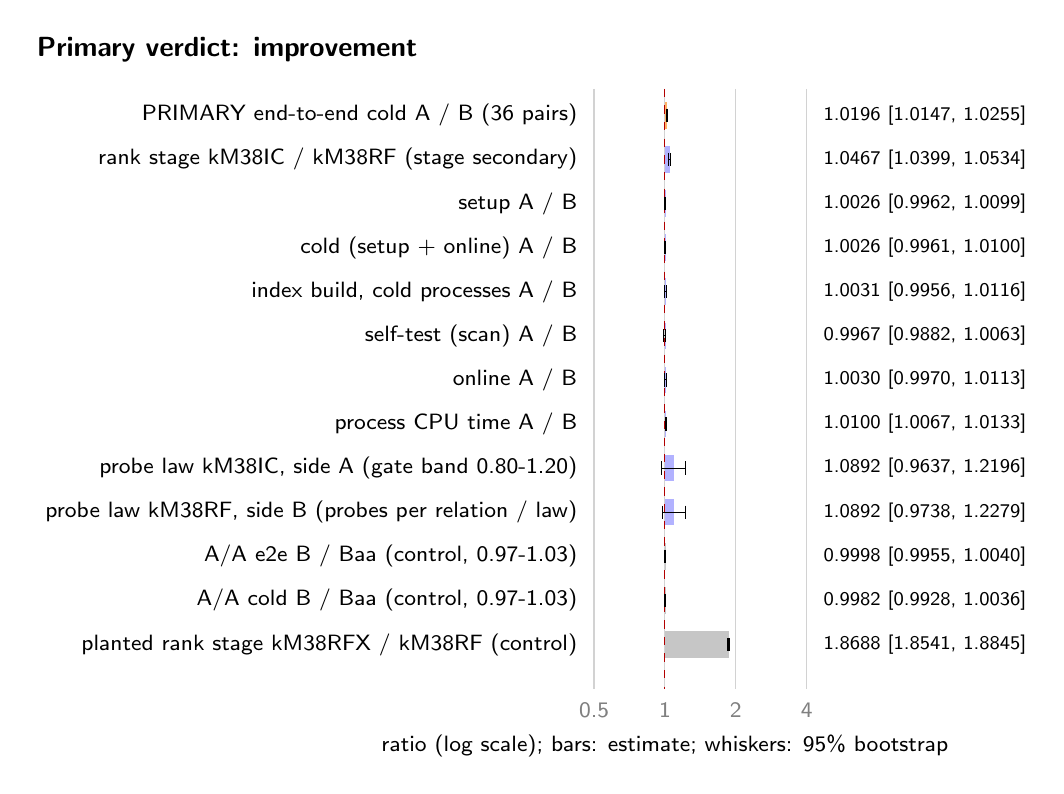
\begin{tikzpicture}[font=\sffamily\footnotesize,x=9mm,y=-5.6mm]
\draw[gray!35] (-1.0000,-0.6) -- (-1.0000,13); \node[gray] at (-1.0000,13.5) {0.5};
\draw[gray!35] (0.0000,-0.6) -- (0.0000,13); \node[gray] at (0.0000,13.5) {1};
\draw[gray!35] (1.0000,-0.6) -- (1.0000,13); \node[gray] at (1.0000,13.5) {2};
\draw[gray!35] (2.0000,-0.6) -- (2.0000,13); \node[gray] at (2.0000,13.5) {4};
\draw[red!70!black,dashed] (0,-0.6) -- (0,13);
\node at (0,14.3) {ratio (log scale); bars: estimate; whiskers: 95\% bootstrap};
\node[anchor=west,font=\sffamily\bfseries] at (-9,-1.5) {Primary verdict: improvement};
\node[anchor=east] at (-1.1000,0) {PRIMARY end-to-end cold A / B (36 pairs)};
\fill[orange!60] (0,-0.300000) rectangle (0.0280,0.300000);
\draw (0.0210,0) -- (0.0363,0); \draw (0.0210,-0.150000) -- (0.0210,0.150000); \draw (0.0363,-0.150000) -- (0.0363,0.150000);
\node[anchor=west,font=\sffamily\scriptsize] at (2.1000,0) {1.0196 [1.0147, 1.0255]};
\node[anchor=east] at (-1.1000,1) {rank stage kM38IC / kM38RF (stage secondary)};
\fill[blue!30] (0,0.700000) rectangle (0.0658,1.300000);
\draw (0.0565,1) -- (0.0751,1); \draw (0.0565,0.850000) -- (0.0565,1.150000); \draw (0.0751,0.850000) -- (0.0751,1.150000);
\node[anchor=west,font=\sffamily\scriptsize] at (2.1000,1) {1.0467 [1.0399, 1.0534]};
\node[anchor=east] at (-1.1000,2) {setup A / B};
\fill[blue!30] (0,1.700000) rectangle (0.0037,2.300000);
\draw (-0.0055,2) -- (0.0143,2); \draw (-0.0055,1.850000) -- (-0.0055,2.150000); \draw (0.0143,1.850000) -- (0.0143,2.150000);
\node[anchor=west,font=\sffamily\scriptsize] at (2.1000,2) {1.0026 [0.9962, 1.0099]};
\node[anchor=east] at (-1.1000,3) {cold (setup + online) A / B};
\fill[blue!30] (0,2.700000) rectangle (0.0038,3.300000);
\draw (-0.0056,3) -- (0.0143,3); \draw (-0.0056,2.850000) -- (-0.0056,3.150000); \draw (0.0143,2.850000) -- (0.0143,3.150000);
\node[anchor=west,font=\sffamily\scriptsize] at (2.1000,3) {1.0026 [0.9961, 1.0100]};
\node[anchor=east] at (-1.1000,4) {index build, cold processes A / B};
\fill[blue!30] (0,3.700000) rectangle (0.0044,4.300000);
\draw (-0.0064,4) -- (0.0166,4); \draw (-0.0064,3.850000) -- (-0.0064,4.150000); \draw (0.0166,3.850000) -- (0.0166,4.150000);
\node[anchor=west,font=\sffamily\scriptsize] at (2.1000,4) {1.0031 [0.9956, 1.0116]};
\node[anchor=east] at (-1.1000,5) {self-test (scan) A / B};
\fill[blue!30] (0,4.700000) rectangle (-0.0047,5.300000);
\draw (-0.0171,5) -- (0.0091,5); \draw (-0.0171,4.850000) -- (-0.0171,5.150000); \draw (0.0091,4.850000) -- (0.0091,5.150000);
\node[anchor=west,font=\sffamily\scriptsize] at (2.1000,5) {0.9967 [0.9882, 1.0063]};
\node[anchor=east] at (-1.1000,6) {online A / B};
\fill[blue!30] (0,5.700000) rectangle (0.0043,6.300000);
\draw (-0.0044,6) -- (0.0162,6); \draw (-0.0044,5.850000) -- (-0.0044,6.150000); \draw (0.0162,5.850000) -- (0.0162,6.150000);
\node[anchor=west,font=\sffamily\scriptsize] at (2.1000,6) {1.0030 [0.9970, 1.0113]};
\node[anchor=east] at (-1.1000,7) {process CPU time A / B};
\fill[blue!30] (0,6.700000) rectangle (0.0143,7.300000);
\draw (0.0097,7) -- (0.0191,7); \draw (0.0097,6.850000) -- (0.0097,7.150000); \draw (0.0191,6.850000) -- (0.0191,7.150000);
\node[anchor=west,font=\sffamily\scriptsize] at (2.1000,7) {1.0100 [1.0067, 1.0133]};
\node[anchor=east] at (-1.1000,8) {probe law kM38IC, side A (gate band 0.80-1.20)};
\fill[blue!30] (0,7.700000) rectangle (0.1233,8.300000);
\draw (-0.0534,8) -- (0.2864,8); \draw (-0.0534,7.850000) -- (-0.0534,8.150000); \draw (0.2864,7.850000) -- (0.2864,8.150000);
\node[anchor=west,font=\sffamily\scriptsize] at (2.1000,8) {1.0892 [0.9637, 1.2196]};
\node[anchor=east] at (-1.1000,9) {probe law kM38RF, side B (probes per relation / law)};
\fill[blue!30] (0,8.700000) rectangle (0.1233,9.300000);
\draw (-0.0383,9) -- (0.2962,9); \draw (-0.0383,8.850000) -- (-0.0383,9.150000); \draw (0.2962,8.850000) -- (0.2962,9.150000);
\node[anchor=west,font=\sffamily\scriptsize] at (2.1000,9) {1.0892 [0.9738, 1.2279]};
\node[anchor=east] at (-1.1000,10) {A/A e2e B / Baa (control, 0.97-1.03)};
\fill[gray!45] (0,9.700000) rectangle (-0.0003,10.300000);
\draw (-0.0064,10) -- (0.0058,10); \draw (-0.0064,9.850000) -- (-0.0064,10.150000); \draw (0.0058,9.850000) -- (0.0058,10.150000);
\node[anchor=west,font=\sffamily\scriptsize] at (2.1000,10) {0.9998 [0.9955, 1.0040]};
\node[anchor=east] at (-1.1000,11) {A/A cold B / Baa (control, 0.97-1.03)};
\fill[gray!45] (0,10.700000) rectangle (-0.0026,11.300000);
\draw (-0.0104,11) -- (0.0051,11); \draw (-0.0104,10.850000) -- (-0.0104,11.150000); \draw (0.0051,10.850000) -- (0.0051,11.150000);
\node[anchor=west,font=\sffamily\scriptsize] at (2.1000,11) {0.9982 [0.9928, 1.0036]};
\node[anchor=east] at (-1.1000,12) {planted rank stage kM38RFX / kM38RF (control)};
\fill[gray!45] (0,11.700000) rectangle (0.9021,12.300000);
\draw (0.8907,12) -- (0.9142,12); \draw (0.8907,11.850000) -- (0.8907,12.150000); \draw (0.9142,11.850000) -- (0.9142,12.150000);
\node[anchor=west,font=\sffamily\scriptsize] at (2.1000,12) {1.8688 [1.8541, 1.8845]};
\end{tikzpicture}
\end{document}
